\chapter{\label{ch:zdcReco}ZDC reconstruction}
  \section{\label{sec:breakUpDet} Nuclear break-up determination}
    As described in Section~\ref{sec:ltaTheory}, UPC \JPsi{} photoproduction 
      can be accompanied by the emission of neutrons from either of the two 
      colliding nuclei.
    The various neutron emission scenarios, or break-up modes, can 
      be distinguished by the two ZDCs.
    By separating events where the ZDC signal is consistent with 1 neutron 
      versus several neutrons, or where neutrons are present on only one or 
      both sides, the fraction of events which corresponds to a given 
      break-up mode can be measured and compared to theory. 

    In order to maximize the ability to explore the one neutron peak, which 
      sits at the bottom of the ZDCs dynamic range, a new ZDC reconstruction 
      method was devised. 
    This new reconstruction method was then used to establish 
      thresholds for one and more than one neutron in each ZDC. 
    This section describes the ZDC signal reconstruction and how the neutron 
      thresholds on this signal were set.
    
    \subsection{ZDC signal reconstruction}
      The signal from each ZDC is built up from the pulse shapes for each of 
        the 18 individual ZDC channels. 
      The pulse shape is recorded in 250 ns second chunks and is divided into
        10 time slices of 25 ns (see Fig~\ref{fig:zdcPulseShape}).
      Counting from 0, the 4th time slice is synced with the timing of the rest
        of the detector and corresponds to when the products of the recorded 
        collision reached the ZDC.
      The signal is therefore taken from the 4th time slice.
      \begin{figure}[h]
        \centering
        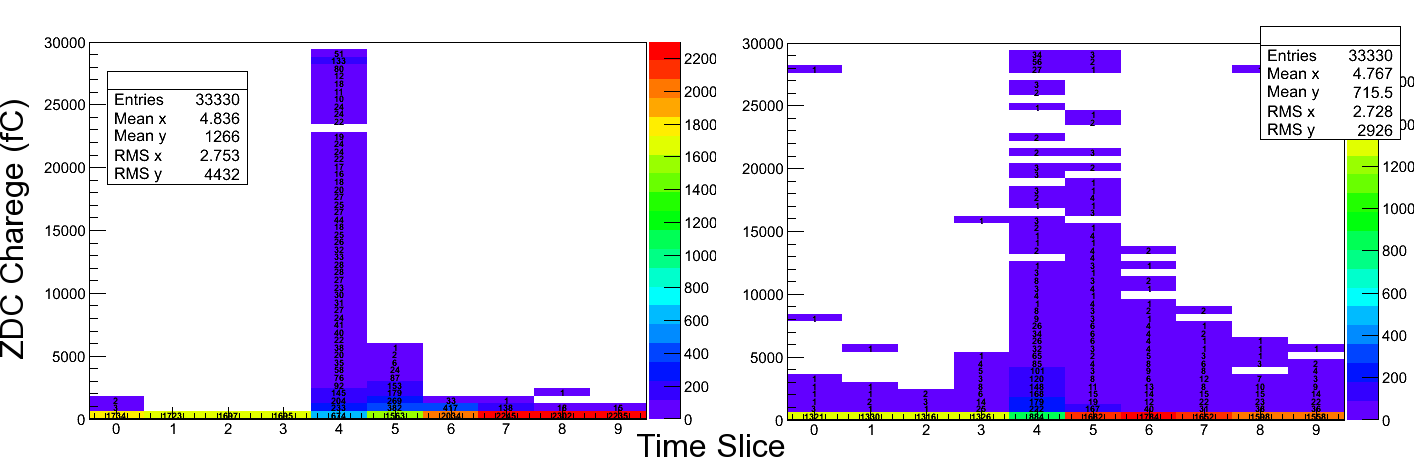
\includegraphics[width=\textwidth]{zdcPulseShape}
        \caption{Average ZDC pluse shape is plotted as the charge as a function
          of time slice for the first hadronic from ZDC$^{-}$ (left) and 
          ZDC$^{+}$ (right).}
        \label{fig:zdcPulseShape}
      \end{figure}

      The ZDC signal sits on top of a low frequency noise pedestal with a 
        period of about 2$\mu$ seconds. 
      Over the time scale of 250 ns, this low frequency noise signal appears
        as a constant that shifts randomly from event to event.
      The contribution from this noise is therefore measured event by event
        in order to subtract it.
      Time slice 5 is used for this purpose.
      Time slices 1 and 2 could also be used to estimate the low frequency 
        noise.
      However because the noise fluctuates to negative values of charge that 
        cannot be measured, these time slices can only provide a 
        measurement of the noise half the time. 
      By using time slice 5 which contains the falling tail of the signal, 
        the noise can be measured any time the signal raises significantly 
        above the noise.
      If the fraction of signal in time slice 4 and 5 are constant and
        the noise contributes the same value to both time slices, the 
        following formula is applicable:
      \begin{equation}
        Ts4 \propto (Ts4 + C) - ( Ts5 + C ) = Ts4 - R_{Ts5/Ts4}Ts4 
        = Ts4(1-R_{Ts5/Ts4}),
        \label{eq:ts4ish}
      \end{equation}
      where $Ts4$ is the signal contribution in time slice 4, $Ts5$ is the 
        signal contribution to time slice 5, $C$ is a random noise constant
        from the low frequency noise, and $R_{Ts5/Ts4}$ is the ratio between
        the signal contribution from time slice 5 over time slice 4.
      Figure~\ref{fig:zdcTs4OvTs5VTs5} demonstrates the consistency of the 
        fraction and validates the unconventional method of using the falling 
        tail of the signal to estimate the low frequency noise. 
      By using time slice 5, the chances of measuring the noise are maximized. 
      Separating the signal from the noise is especially important because
        the ZDC signal for the one neutron peak sits near the noise at the 
        bottom of the ZDC dynamic range.
      \begin{figure}[!Hhbt]
        \centering
        $ \begin{array}{cc}
          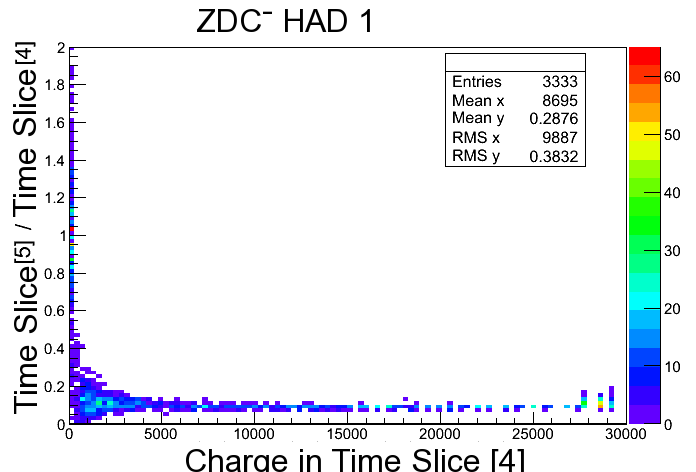
\includegraphics[width=.4\textwidth]{negTs5overTs4vts5} &
          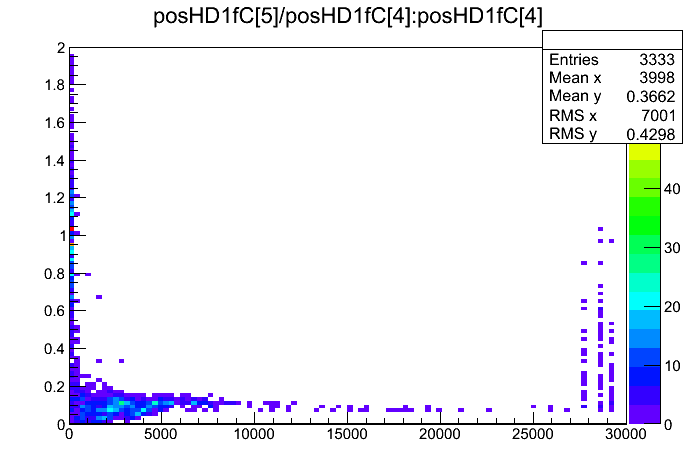
\includegraphics[width=.4\textwidth]{posTs5overTs4vts5}
        \end{array} $  
        \caption{ The fraction of signal in time slice 5 over time slice 4 
          as a function of the signal in time slice 5 in ZDC$^{-}$ (left) and 
          ZDC$^{+}$ (right).}
        \label{fig:zdcTs4OvTs5VTs5}
      \end{figure}
      
      When summing the 9 channels in each ZDC, only channels with signals above 
        zero in time slices 4 and 5 were included. 
      The EM, electromagnetic, section of the calorimeter is more densely 
        packed with quartz fibers and therefore has a higher gain relative to 
        the HAD, hadronic, section. 
      To account for this, the EM channels were weighted with
        a factor of 0.1 to match the HAD channel gains.

    \subsection{Determination of the one neutron thresholds}
      The ZDC thresholds used to establish the various break-up modes were 
        measured from zero bias data.
      Figure~\ref{fig:zdcM2Fit} shows the weighted sum of the EM and 
        HAD sections for  ZDC$^{-}$ and  ZDC$^{+}$ for the zero bias 
        dataset.
      The neutron spectrum for this dataset is not biased since the 
        trigger only required that both beams were present in CMS. 
      This dataset does, however, include a significant electronic noise contribution due
        to events where no neutrons are emitted in the direction of the ZDC.
      It is clear from Fig.~\ref{fig:zdcM2Fit} that the gain of  
        ZDC$^{+}$ is lower than that of ZDC$^{-}$. 
      This is because of a damaged phototube on the first HAD section 
        of ZDC$^{+}$.

      To determine the thresholds for one and multiple neutrons, the ZDC$^{+}$ 
        and ZDC$^{-}$ spectra were 
        each fit to the sum of four Gaussians. 
      The electronic pedestal noise was fit to a Gaussian around zero.
      The one, two, and three neutron peaks are fit to Gaussians that are 
        successively broader.
      The mean of each peak was initially set to multiples of the mean of the 
        one neutron peak. 
      \begin{figure}[!Hh]
        \centering
        $
          \begin{array}{cc}
            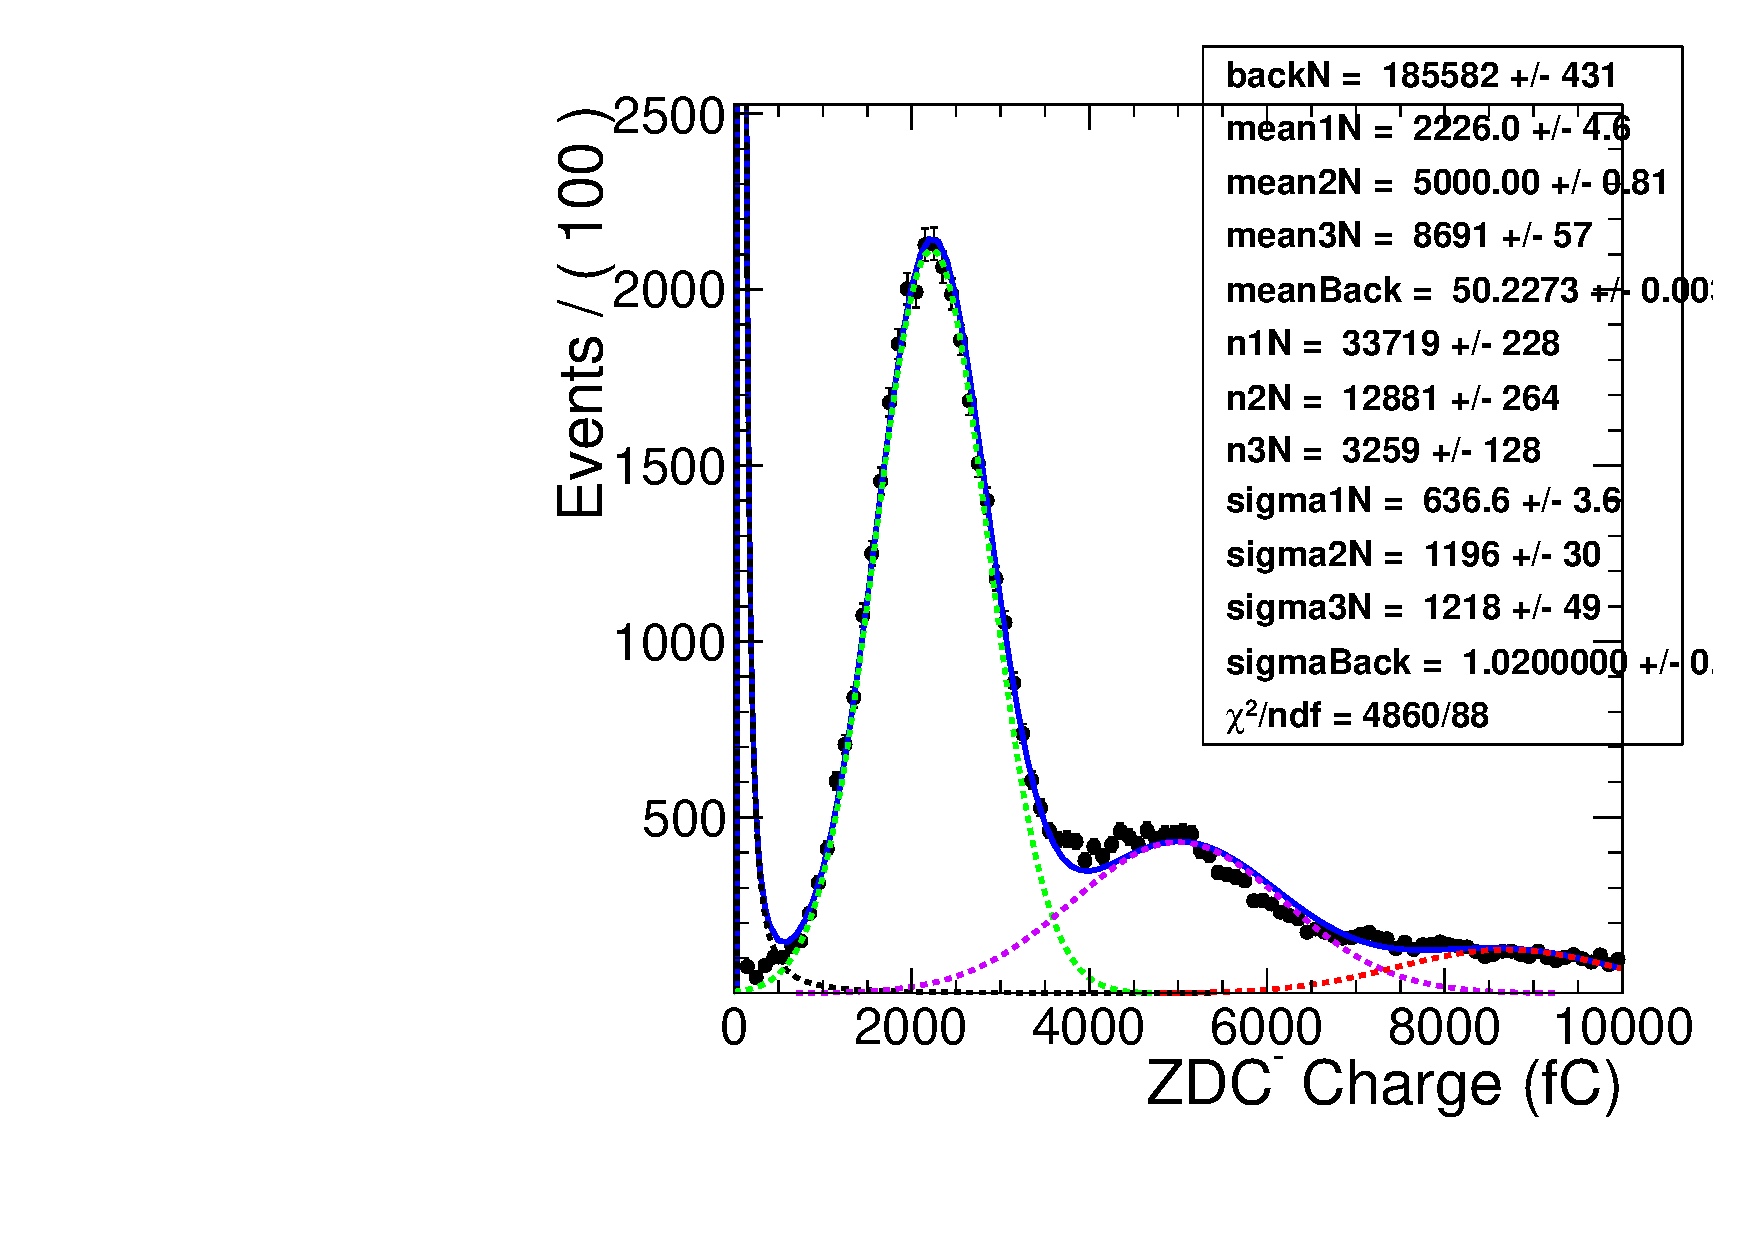
\includegraphics[width=0.45\textwidth]{zdcFit45Neg.pdf} &
            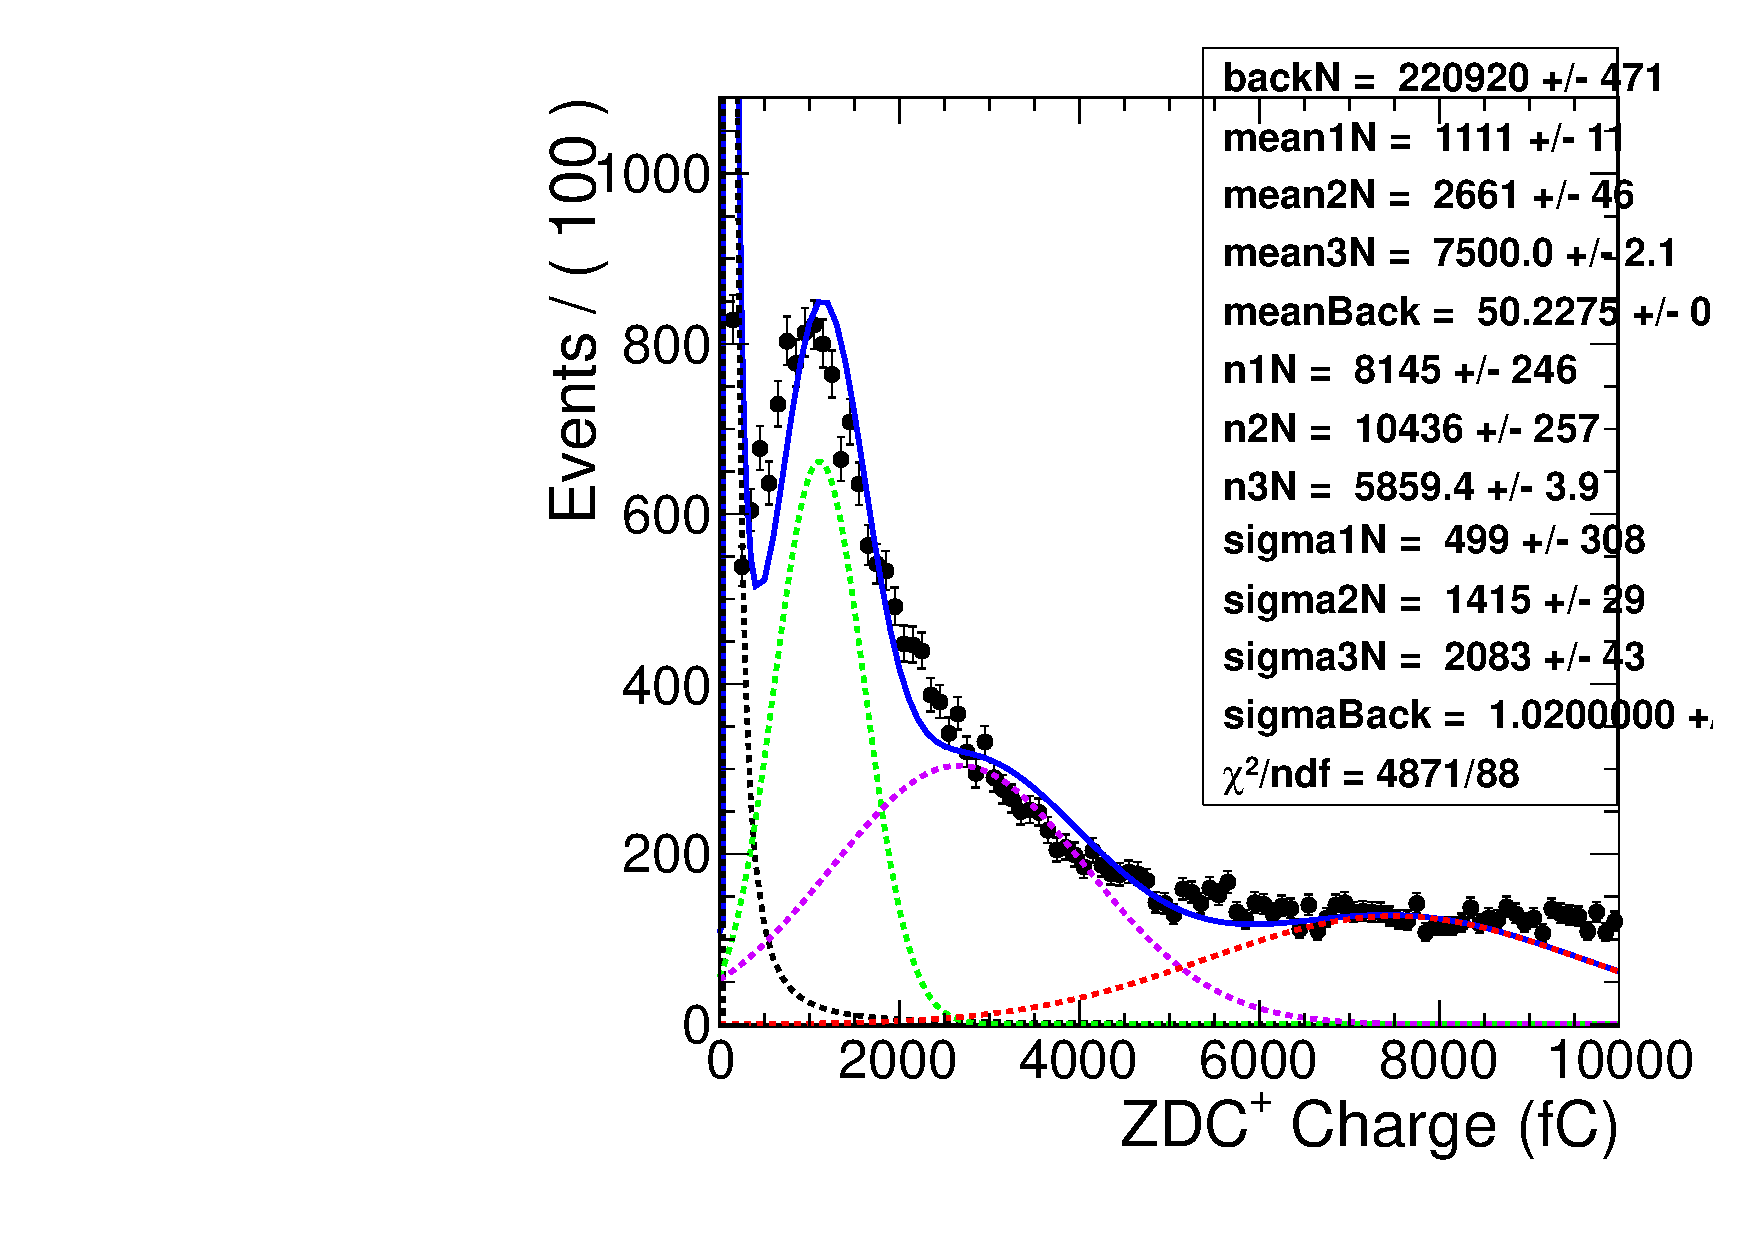
\includegraphics[width=0.45\textwidth]{zdcFit45Pos.pdf}
          \end{array} 
        $
        \caption{Fit to the signal spectra for ZDC$^{-}$ (left) and ZDC$^{+}$ 
          (right)}
        \label{fig:zdcM2Fit}
      \end{figure}
      The threshold for a neutron in the ZDC was taken from the fits in 
        Fig.~\ref{fig:zdcM2Fit}.
      Any signal greater 2$\sigma$ below the mean of the one neutron peak was 
        considered signal.
      Any signal greater than 2$\sigma$ above was considered multiple 
        neutrons.
      The single neutron break up modes were separated from the multiple 
        neutron modes by use of these definitions.

      Several of the break-up mode calculations that have been done involve
        single sided configurations where neutrons are present on one side
        of the interaction point and not the other.
      These modes can be hard to identify because the single neutron peak in 
        ZDC$^{+}$ overlaps with the noise peak at zero.
      To identify events where the ZDCs only measured noise, the noise
        spectra were measured directly.
      Placing an additional criteria based on the ZDCs noise distributions for
        when the ZDCs are devoid of signal provides assurance that the events 
        tagged as single sided events are truly single sided.

      
      The noise distributions for the EM sections and the HAD sections were
        measured separately from out of time time slices.
      In Fig.~\ref{fig:zdcPulseShape} higher than average signal can be seen
        in the 0th time slice, which precedes the main signal time slice 
        time slice 4 by 200 ns. 
      This is due to events where activity was present in the ZDC for 
        two consecutive collisions.
      Time slices 1 and 2, however, occurred between collisions.
      These time slices, which occur out of time, were used to measure the 
        noise spectrum.
      \begin{figure}[!Hhbt]
        \centering
        $ \begin{array}{cc}
          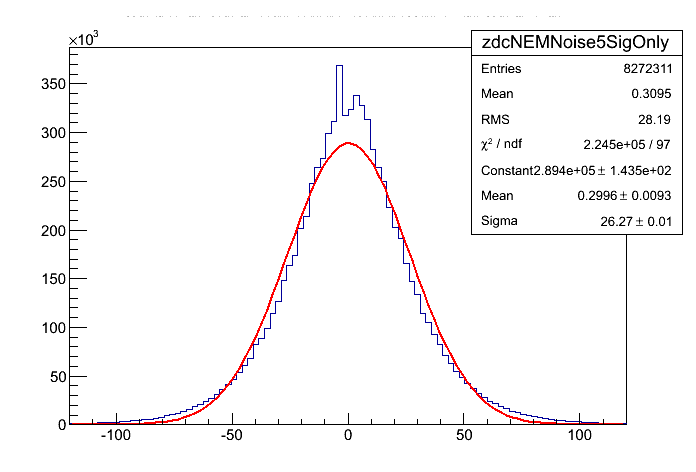
\includegraphics[width=.45\textwidth]{zdcNegEMNoiseFromZBNoCor} & 
          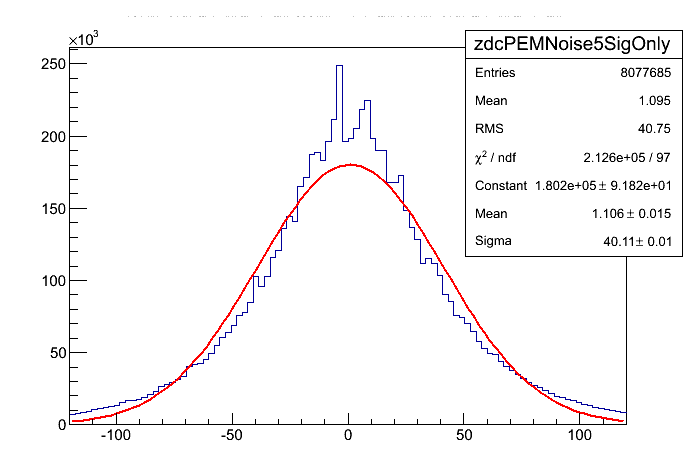
\includegraphics[width=.45\textwidth]{zdcPosEMNoiseFromZBNoCor} \\
          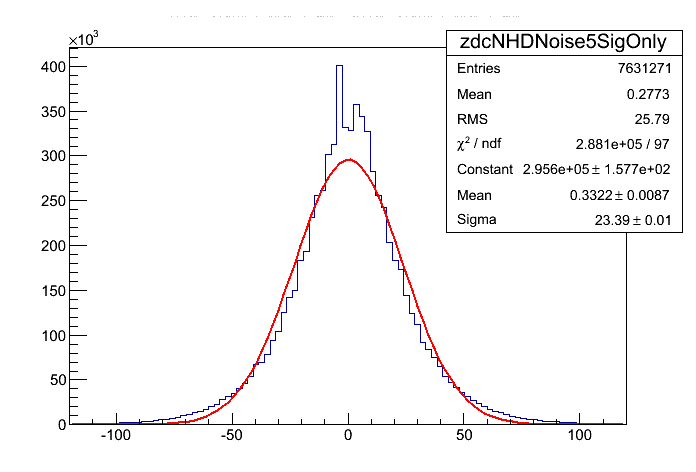
\includegraphics[width=.45\textwidth]{zdcNegHDNoiseFromZB} &
          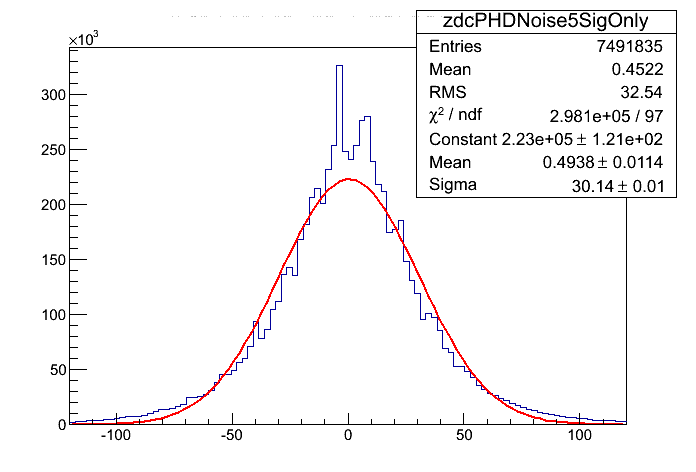
\includegraphics[width=.45\textwidth]{zdcPosHDNoiseFromZB}
        \end{array} $
        \caption{ZDC noise spectra from ZDC$^{-}$ EM section (upper left), 
          ZDC$^{+}$ EM section (upper right), ZDC$^{-}$ HAD section (lower left), 
          and ZDC$^{+}$ HAD section (lower right) from out of time time slices.}
        \label{fig:zdcNoiseSpectra}
      \end{figure}

      As with the signal measurements, the low frequency noise pedestal is 
        subtracted event by event by subtracting time slice 2 from time slice
        1 leaving only the high frequency noise.
      The noise distributions do not depend on the amount of quartz fibers, but
        because the signal does, the noise distributions for EM and HAD sections
        are measured separately.
      Figure~\ref{fig:zdcNoiseSpectra} shows the noise spectrum for each of the 
        EM and HAD sections for the two ZDCs.
      If the HAD or EM signals measured from time slices which match the 
        timing for a collision, time slices 4 and 5, are less than 2$\sigma$ 
        above the mean of the noise distribution or lower, these sections are 
        considered consistent with noise.
      A ZDC is considered consistent with noise if both the HAD section and EM 
        section from that ZDC have signal measurements consistent with noise.

    \subsection{\label{sec:zdcCompare}ZDC reconstruction method comparison}
      In this section the nominal ZDC reconstruction method designed for this
        thesis is compared to an alternative method.
      This additional method, used in previous ZDC measurements, differs 
        in the way the signal time slices are used to calculate the signal from
        each channel.
      In the additional alternative method, the signal is taken from the sum of 
        time slices 4, 5, and 6.
      To estimate the event by event noise pedestal the sum of time slice 
        1 and 2 are used. 
      The signal for an individual ZDC channel is then calculated as the 
        sum of the signal time slices minus the sum of the noise time slices
        weighted by a factor of 3/2 to account for the differing number of 
        noise versus signal time slices.
      As in the nominal method described in Section~\ref{sec:breakUpDet}, 
        the alternative method combines the channels to create a signal 
        measurement from the whole of each side of the ZDC, one
        measurement for ZDC$^{+}$, and one for ZDC$^{-}$.
      The noise subtracted signal from each of the HAD channels are added 
        together.
      Then the EM section channels are summed. 
      The EM section is weighted by a factor of 0.1 as in the nominal method. 
      After the weighting the EM and HAD channels are added to each to create
        one measurement for ZDC$^{+}$ and another measurement for ZDC$^{-}$.
      Figure~\ref{fig:zdcM1Fit} shows the spectra for ZDC$^{+}$ and ZDC${-}$ 
        using the alternative method. 
      The same fit used for the nominal method is applied to the alternative 
        method. 
      As in the nominal method, the single neutron threshold is set to 2$\sigma$
        below the mean from the fit to the one neutron peak.
      The multi-neutron threshold was set to 2$\sigma$ above the one neutron
        peak.
      \begin{figure}[!Hhtb]
        \centering
        $ \begin{array}{cc}
          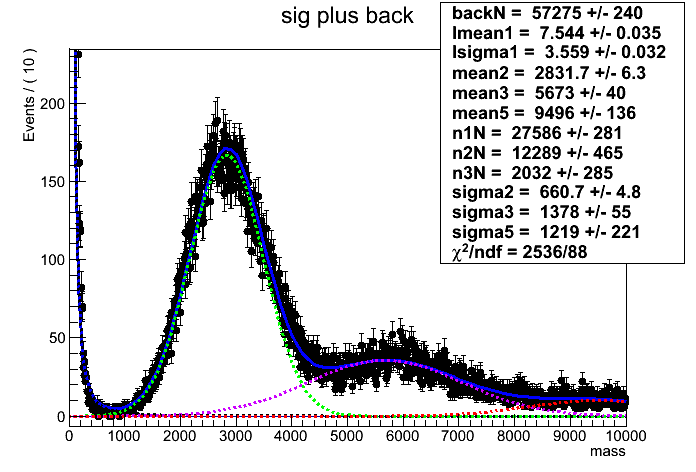
\includegraphics[width=0.45\textwidth]{zdcMinusZBFitTimeCut} &
          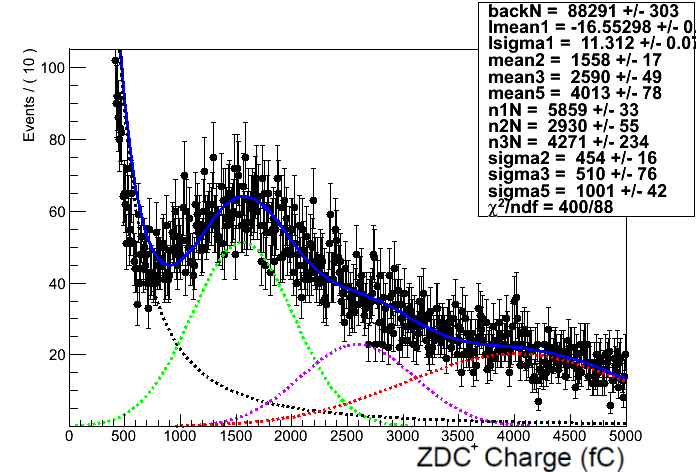
\includegraphics[width=0.45\textwidth]{zdcPlusZBFitTimeCut}
        \end{array} $
        \caption{Fit to charge spectrum from ZDC$^{-}$ (left) and ZDC$^{+}$ 
          (right) using the alternative reconstruction method}
        \label{fig:zdcM1Fit}
      \end{figure}

      The advantage of the alternative method is that by using multiple signal
        and noise time slices the signal and noise are effectively averaged
        reducing time slice to time slice fluctuations.
      However, by using time slices 1 and 2 for measuring the noise, the noise
        can only be measured half the time due to unmeasurable negative 
        fluctuations of the dominant low frequency component of the noise.
      The nominal method relative to the alternative method separates low signal
        from the noise more effectively  for both sides of the ZDC.
      This is particularly important for ZDC$^{+}$ where the 1st HAD section
        had a lower gain than the other sections. 
      The ZDC$^{+}$ and ZDC$^{-}$ signals near the one neutron peak using the
        alternative and nominal reconstruction methods were plotted for comparison in 
        Fig.~\ref{fig:zdcSpec2v1}.
      \begin{figure*}[!Hhbt]
        \centering
        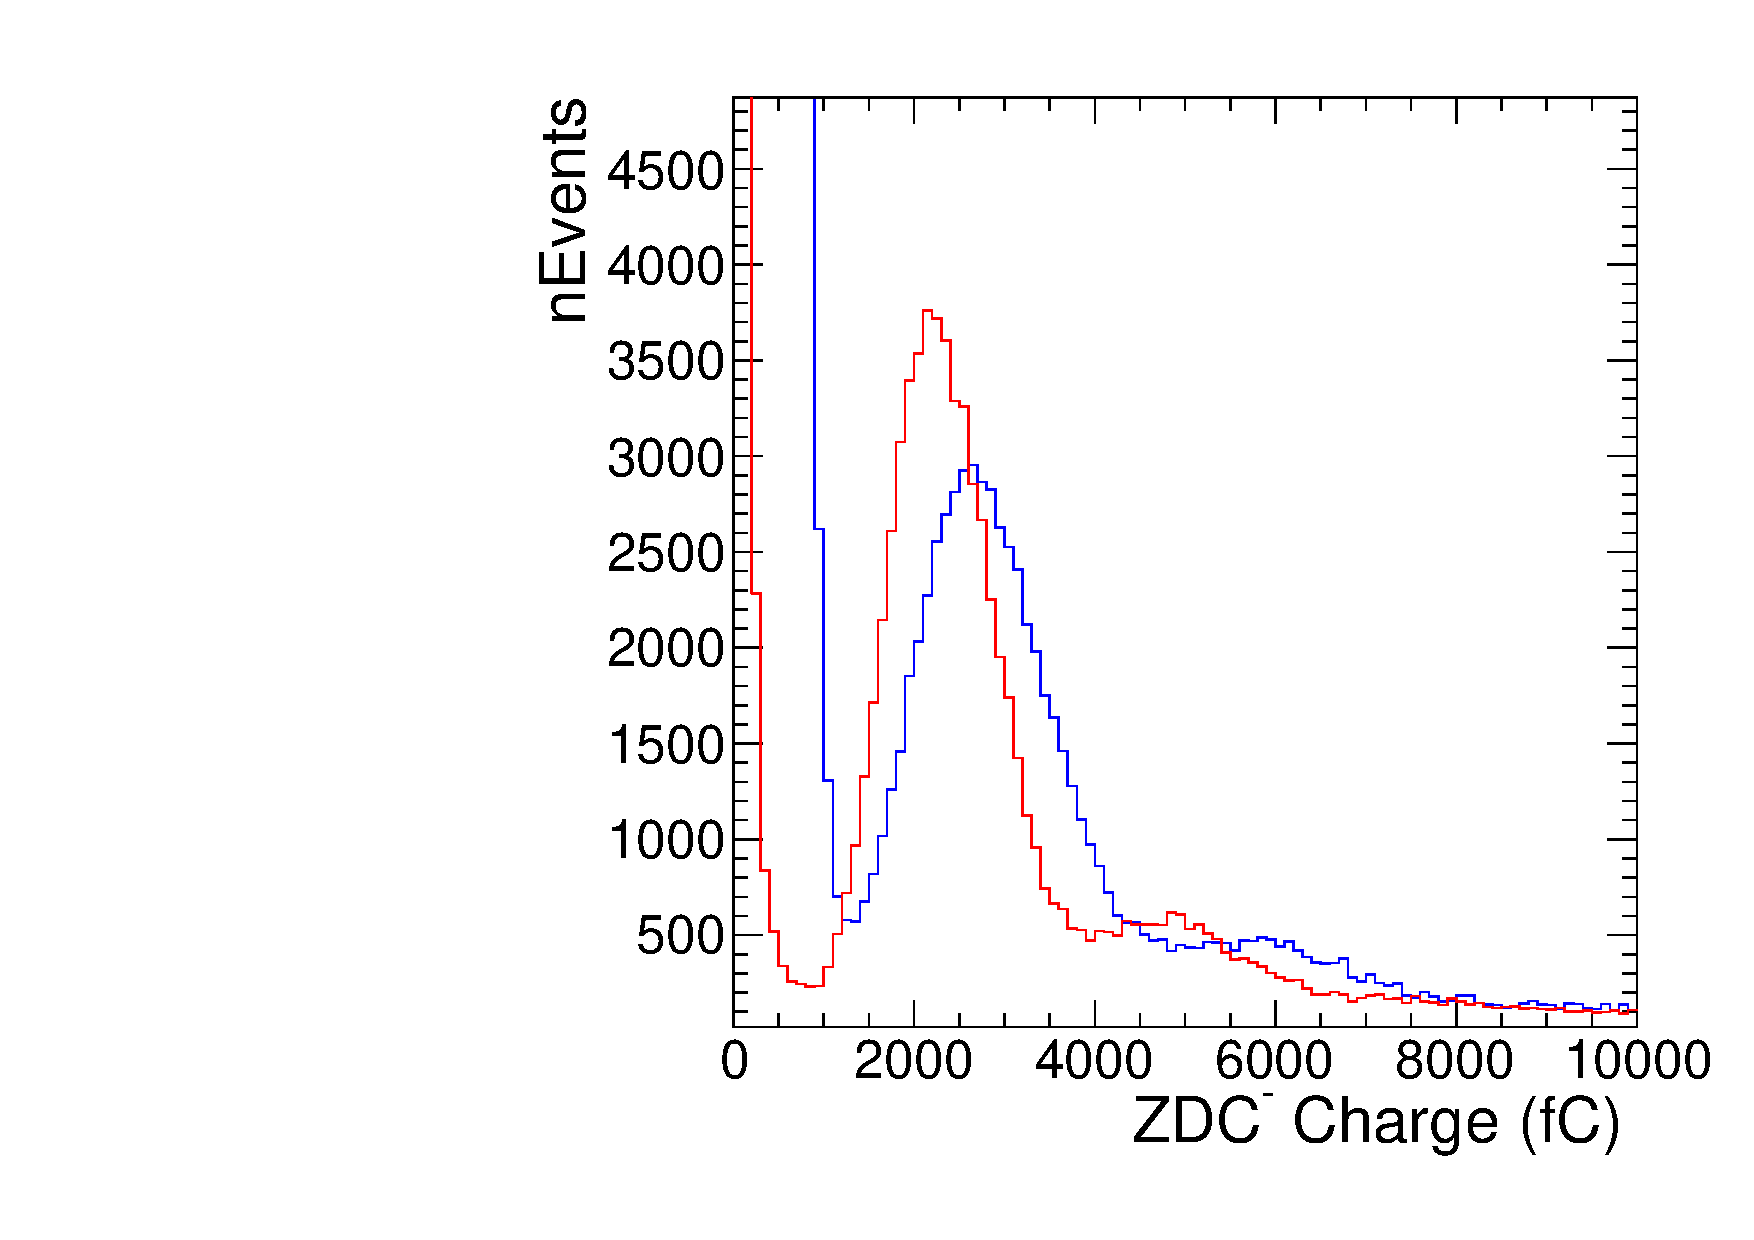
\includegraphics[width=.45\textwidth]{zdcSpec2v1Minus}
        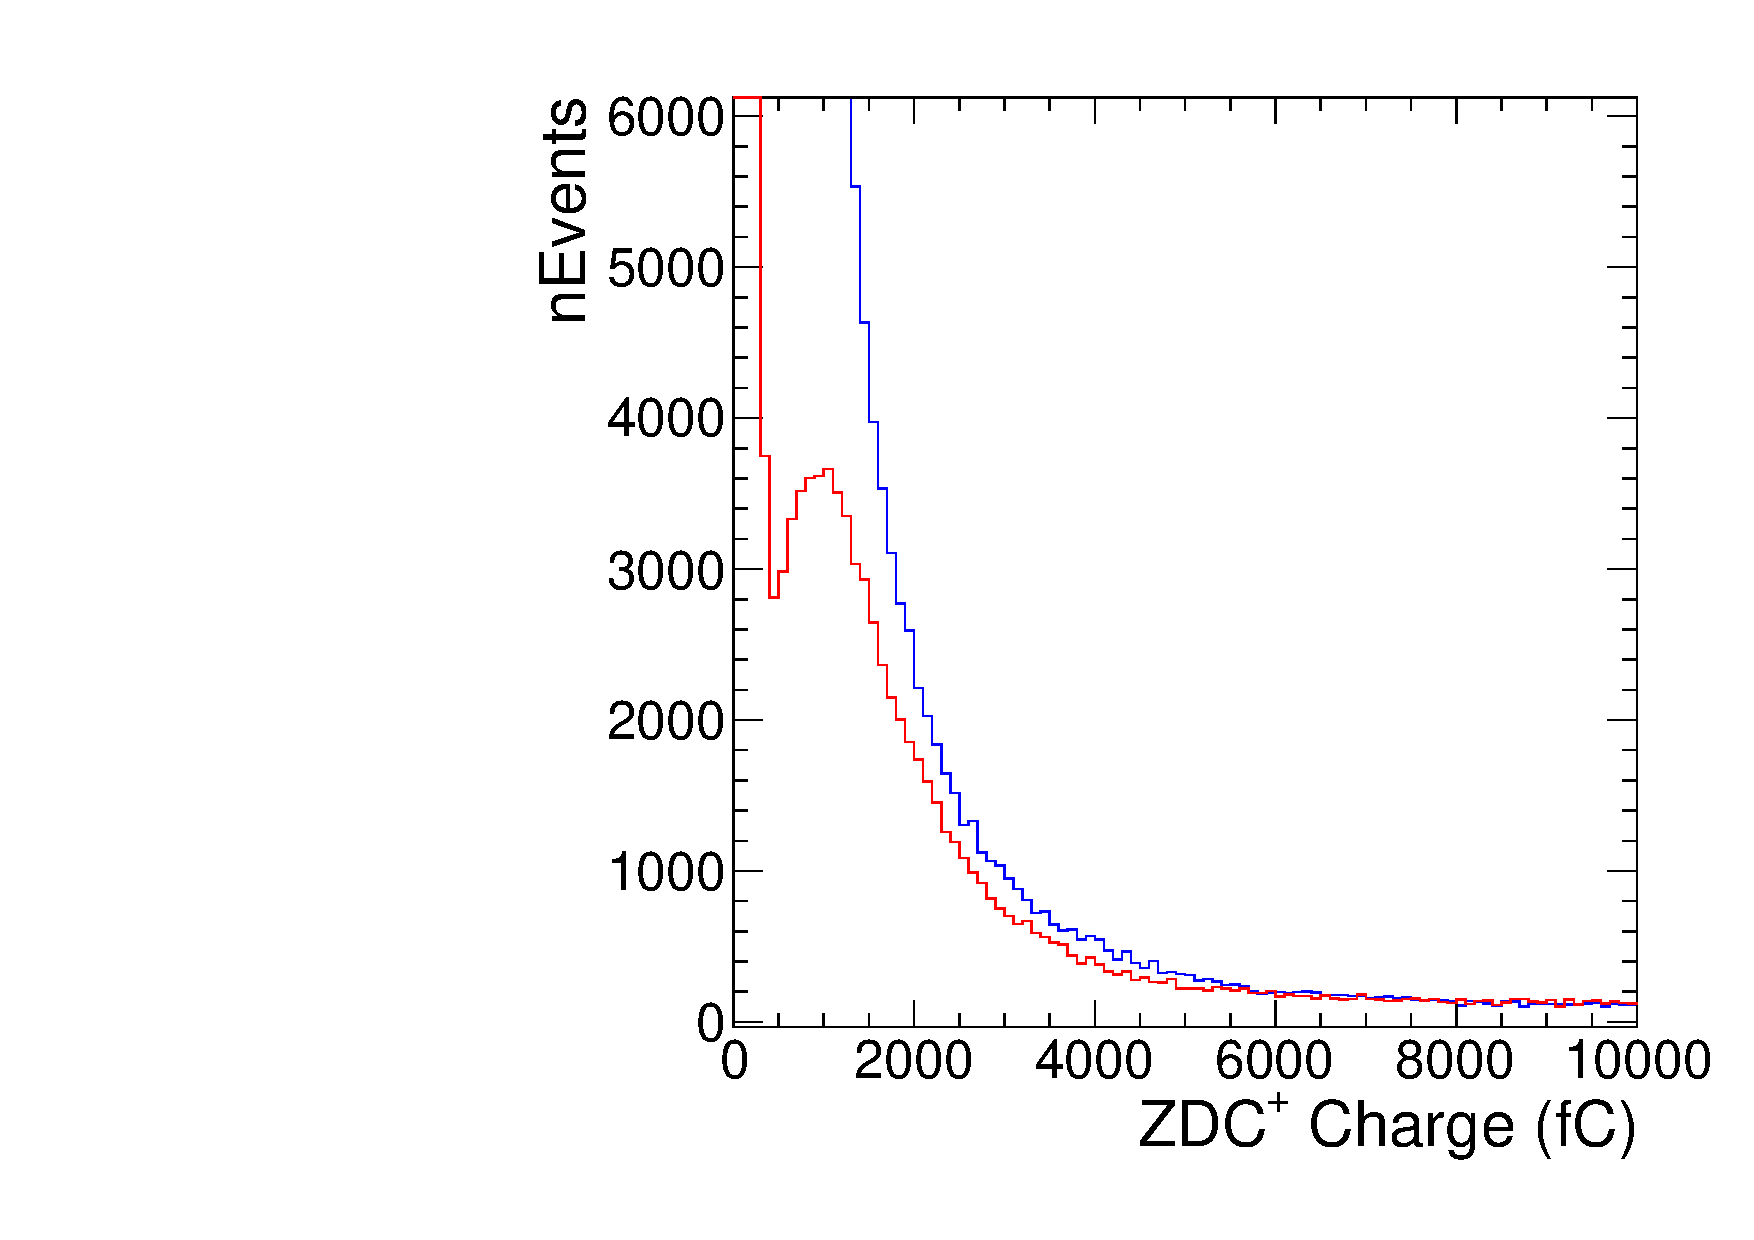
\includegraphics[width=.45\textwidth]{zdcSpec2v1Plus}
        \caption{Comparison of the nominal (red) ZDC reconstruction 
          method and the alternative (blue) method for ZDC$^{-}$ (left) and 
          ZDC$^{+}$ (right).}
        \label{fig:zdcSpec2v1}
      \end{figure*}
      In Fig.~\ref{fig:zdcSpec2v1}, the shrinking of width of the noise peak 
        around zero in the nominal method versus the old method is apparent for
        both ZDC$^{+}$ and ZDC$^{-}$.
      For the alternative method no single neutron peak is resolved in ZDC$^{+}$,
        whereas the single neutron peak is resolved using the nominal method. 

      Timing cuts were applied to enhance the signal relative to the background
        in order to resolve the one neutron peak in ZDC$^{+}$ using the 
        alternative method. 
      Because the products of the collision are synced with time slice 4, noise
        can be rejected by selecting channels where the maximum signal falls 
        into time slice 4.
      The noise will have no preferred time slice (see Fig.~\ref{fig:zdcPulseShape}). 
      Using this fact, neutron events can be selected by requiring that the
        hadronic channels of the ZDC have a peak signal in the fourth time 
        slice.
      Through these timing cuts the single neutron peak was recovered using the
       alternative reconstruction for ZDC$^{+}$.

      To examine the effectiveness of the timing cuts, event by event noise 
        subtraction was removed from the alternative reconstruction.
      The signal from each channel was taken from time slices 4,5, and 6 with
        out subtracting 1 and 2.
      The signal spectrum from ZDC$^{-}$ was then plotted with the result
        shown in Fig.~\ref{fig:zdcTimingCuts}.
      \begin{figure}[!Hhbt]
        \centering
        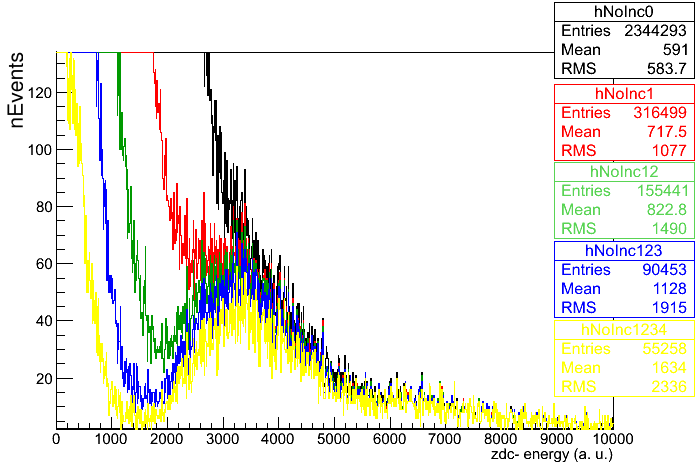
\includegraphics[width=0.6\textwidth]{zdcMinusSingleNuNoInc}
        \caption{Effects of requiring in-time signal in successively more 
          ZDC$^{-}$ hadronic channels, no timing, at least one (red), at least two (green),
            at least three (blue), and all four (yelow) HAD channels have a maximum signal
            in the fourth time slice.}
        \label{fig:zdcTimingCuts}
      \end{figure}
      As each additional hadronic channel is required to have a maximum signal
        in the fourth time slice, the single neutron peak emerges. 
      Figure~\ref{fig:zdcTimingCuts} demonstrates that the single neutron peak 
        can be recovered from the noise using timing cuts alone. 

      Using the alternative noise subtraction method, the same signal that emerges
        from the timing cuts alone appear without timing cuts.
       \begin{figure}[h]
        \centering
        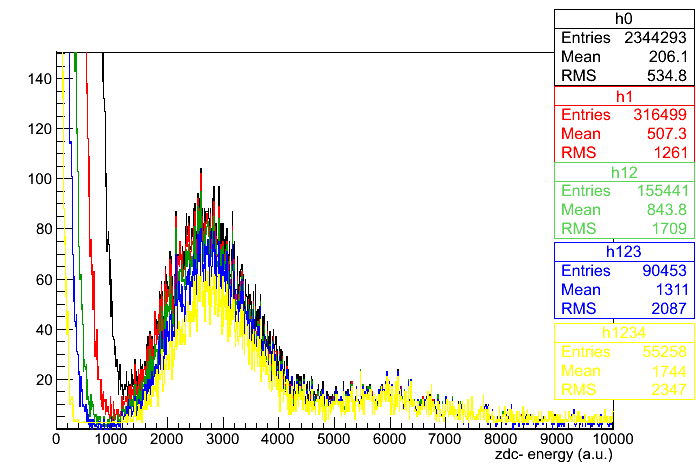
\includegraphics[width=0.6\textwidth]{zdcMinusSingleNuNoSub}
        \caption{Effect of ZDC signal timing requirements after noise 
          subtraction.}
        \label{fig:zdcTimingAfterNoiseSub}
      \end{figure}
      Figure~\ref{fig:zdcTimingAfterNoiseSub} confirms that both noise 
        subtraction and the timing requirement produce the same signal.
      This gives confidence that the signal is not an artifact of either cut, 
        but the true neutron signal.

      Figure~\ref{fig:zdcTimingAfterNoiseSub} and Fig.~\ref{fig:zdcTimingCuts} 
        demonstrate the consistency of using timing cuts and noise 
        subtraction to enhance the signal neutron peak. 
      Figure~\ref{fig:zdcTimingAfterNoiseSub} confirms the legitimacy of the 
        timing requirement method in ZDC$^{-}$ by showing that the same
        signal emerges from the noise subtraction method as the timing method.
      Fig.~\ref{fig:zdcSpec2v1} demonstrates the correspondence between
        the nominal noise subtraction method and the alternative method in 
        ZDC$^{-}$ where the signal is better separated from the electronic noise. 
      This provides confidence that the signal seen in ZDC$^{+}$ using 
        the nominal method is the one neutron peak.
